%% Методические указания к выполнению, оформлению и защите выпускной квалификационной работы бакалавра
%% 2.5 Конструкторский раздел
%%
%% В конструкторском разделе описывается разрабатываемый и/или модифицируемый метод или алгоритм.
%%
%% В случае если в бакалаврском проекте разрабатывается новый метод или алгоритм, необходимо подробно изложить их суть, привести все необходимые для их реализации математические выкладки, обосновать последовательность этапов выполнения.
%% При этом для каждого этапа следует выделить необходимые исходные данные и получаемые результаты.
%%
%% При использовании известного алгоритма следует указать специфические особенности его практической реализации, присущие решаемой задаче, и пути их решения в ходе программирования.
%% Для описания метода или алгоритма необходимо выбрать наиболее подходящую форму записи (схема (ГОСТ 19.701-90), диаграмма деятельности, псевдокод и т. п.).
%% Учитывая, что на эффективность алгоритма непосредственно влияют используемые структуры данных, в данном разделе РПЗ целесообразно провести сравнительный анализ структур, которые могут быть применены в рамках программной реализации выбранного алгоритма, и обосновать выбор одной из них.
%% В конце описания разработанного и/или модифицируемого алгоритма должны быть приведены выбранные способы тестирования и сами тесты.
%%
%% Перед формированием тестовых наборов данных целесообразно указать выделенные классы эквивалентности.
%% В данной части расчётно-пояснительной записки могут также выполняться расчёты для определения объёмов памяти, необходимой для хранения данных, промежуточных и окончательных результатов работы программы, а также расчёты, позволяющие оценить время решения задачи на ЭВМ.
%% Эти результаты могут использоваться для обоснования правильности выбора метода и/или алгоритма из имеющихся альтернативных вариантов, а также для оценки возможности практически реализовать поставленную задачу на имеющейся технической базе.
%%
%% Другой важный момент, который должен найти свое отражение в конструкторском разделе, это описание структуры разрабатываемого программного обеспечения.
%% Обычно оно включает в себя:
%% — описание общей структуры — определение основных частей (компонентов) и их взаимосвязей по управлению и по данным;
%% — декомпозицию компонентов и построение структурных иерархий;
%% — проектирование компонентов.
%%
%% Для графического представления такого описания, если есть необходимость, следует использовать:
%% — функциональную модель IDEF0 с декомпозицией решения исходной задачи на несколько уровней (разрабатываемые модули обычно играют роль механизмов);
%% — спецификации компонентов (процессов);
%% — модель данных (ER-диаграмма);
%% — диаграмму классов;
%% — диаграмму компонентов;
%% — диаграмму переходов состояний (конечный автомат), характеризующих поведение системы во времени.
%%
%% Рекомендуемый объём конструкторского раздела 25—30 страниц.

\chapter{Конструкторский раздел}

\section{Моделирование геометрии поверхностей сред}

По описанным в аналитическом разделе ограничениям в качестве объектов в моделируемой световой системе рассматриваются цилиндрические симметрии: бесконечные (по оси Z) цилиндр и эллиптический цилиндр.

Формы оболочек таких сред описывают распространённые до трёхмерного пространства уравнения окружности и эллипса.

Цилиндр задаётся центром $\vec C$ и радиусом $R$:

\begin{equation}
	\label{eqn:cylinder}
	(x - C_x)^2 + (y - C_y)^2 = R^2,
\end{equation}

Эллиптический цилиндр~— центром $\vec C$, длиной большой оси $2a$ и малой — $2b$:

\begin{equation}
	\label{eqn:elliptic-cylinder}
	\frac{(x - C_x)^2}{a^2} + \frac{(y - C_y)^2}{b^2} = 1.
\end{equation}

Для моделирования неоднородности по объёму распределения оптических свойств среды и температуры столб вещества или материала равномерно разбивается на некоторое заданное количество $N_p$ концентрических цилиндрических симметрий, в пределах которых температура и коэффициент оптического поглощения считаются постоянными.
Поэтому для более точных результатов моделирования необходимо задавать достаточное количество разбиений $N_p$.

\section{Моделирование геометрии объёмного излучения}

Для трассировки траектории фотона необходимо помимо начального положения определить и его направление.
Световое излучение представляет собой сферическую волну, поэтому генерация направлений распространения фотонов аналогична задаче генерации точек на поверхности сферы.

Первая мысль, которая приходит в голову,~— попытаться равномерно распределить точки на сфере. Задача о равномерном распределении точек на сфере имеет довольно длительную историю и, к сожалению, за исключением немногочисленного количества частных случаев не имеет точного решения.

Из всех приближённых методов генерации равномерно распределённых по сфере точек наиболее простым и в то же время довольно действенным способом является метод, основанный на решётке Фибоначчи, или, по-другому,~— на золотой спирали.

Вместе с тем, решётка Фибоначчи — это один из малочисленных способов генерации, позволяющих построить сферу из произвольно заданного числа точек $n$.

Спираль Фибоначчи квазиравномерно распределяет $n$ точек в пределах единичного квадрата $[0, 1)^2$ по следующей формуле:

\begin{equation}
	t_i = (x_i, y_i) = \left(\left\{\frac{i}{\varphi}\right\}, \frac{i}{n}\right) \text{ для } 0 \leqslant i < n,
\end{equation}

\noindent где $\varphi$ — золотое сечение, а оператор фигурные скобки обозначает взятие дробной часть аргумента.

Далее, множество точек в пределах единичного квадрата $[0, 1)^2$ накладывается на единичную сферу $S^2$ с помощью цилиндрического равноплощадного проецирования:

\begin{align}
	(x, y) \to (\theta, \phi)&\colon (2 \pi x, \arccos{(1 - 2y)}, \\
	(\theta, \phi) \to (x, y, z)&\colon (\cos\theta \sin\phi, \sin\theta \sin\phi, \cos\phi),
\end{align}

\noindent где $\theta \in [0, 2\pi]$ — долгота, а $\phi \in [0, \pi]$ — угол от условного севера в сферической системе координат.

Преимущество такого способа генерации светового излучения состоит в том, что по каждому направлению объёмная интенсивность будет примерно одинаковая.

Другой подход, более точный, заключается в генерации каркасной сетки на сфере по меридианам и широтам:

\begin{equation}
	\begin{cases}
		x = \sin{\left(\pi \cdot \frac mM\right)}\cos{\left(2\pi \cdot \frac nN\right)}, \\
		y = \sin{\left(\pi \cdot \frac mM\right)}\sin{\left(2\pi \cdot \frac nN\right)}, \\
		z = \cos{\left(\pi \cdot \frac mM\right)}, \\
		m = \{0, \ldots, M\}, n = \{0, \ldots, N-1\},
	\end{cases}
\end{equation}

\noindent где $M$ — количество широт, $N$ — меридианов.

При таком способе объёмная интенсивность фотонов неравномерна и зависит от переменного телесного угла:


\begin{equation}
	\mathrm{d}\Omega = \sin{\theta} \, \mathrm{d}\theta \, \mathrm{d}\phi,
\end{equation}

\noindent где $\displaystyle \theta = \frac{\pi}{M}$, $\displaystyle \phi = \frac{2\pi}{N}$.

На рисунке \ref{img:fibonacci-and-wire-spheres} — визуализация двух способов генерации точек на сфере.

\begin{figure}[ht]
	\center{
		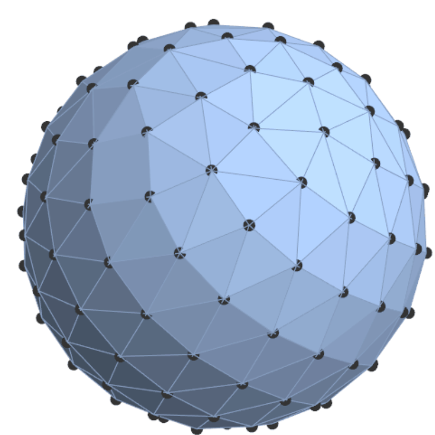
\includegraphics[height=80mm]{inc/img/fibonacci-sphere}
		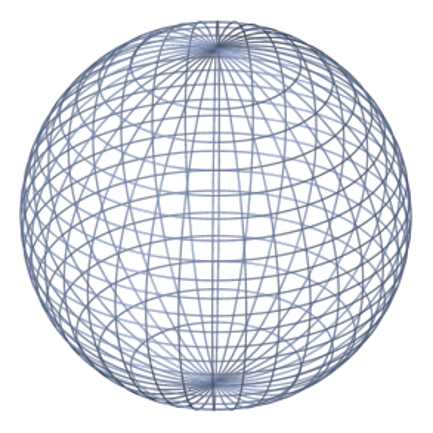
\includegraphics[height=80mm]{inc/img/wire-sphere}
	}
	\captionsetup{justification=centering}
	\caption{Сетка Фибоначчи и каркасная сетка}
	\label{img:fibonacci-and-wire-spheres}
\end{figure}

\section{Моделирование траектории луча}

Луч — это часть прямой, состоящая из заданной точки (начала) и всех точек, лежащих по определённую сторону от неё.
В настоящей работе удобнее задавать луч вектором начала $\vec P = (P_x, P_y, P_z)$ и направления $\vec D = (D_x, D_y, D_z)$.
В таком случае уравнение луча в трёхмерном пространстве имеет параметрический вид:

\begin{equation}
	\vec R = \vec P + \vec D \cdot t, \; t \geqslant 0.
\end{equation}

При достижении границы раздела двух сред прямолинейная траектория луча меняется, часть луча отражается, часть — преломляется.

Результирующий луч согласно закону зеркального отражения рассчитывается по формуле:

\begin{equation}
	\label{eqn:reflection}
	\vec R = \vec I = 2\left(\vec I \cdot \vec N\right)\vec N,
\end{equation}

\noindent где $\vec I$ — луч падающий, а $\vec N$ — нормаль к поверхности в точке падения.

Закон Снеллиуса в векторной форме задаёт координаты преломлённого луча:

\begin{equation}
	\label{eqn:refraction-begin}
	\mu = \frac{\eta_i}{\eta_t},
\end{equation}
\begin{equation}
	\label{eqn:snells-law-g}
	g = \sqrt{1 - \mu^2\left(1 - \left(\vec I \cdot \vec N\right)\right)^2},
\end{equation}
\begin{equation}
	\vec T = g \vec N + \mu \left(\vec I - \left(\vec I \cdot \vec N\right) \vec N\right),
\end{equation}

\noindent где $\eta_i$, $\eta_t$ — показатели преломления сред падающего $\vec I$ и преломлённого $\vec T$ лучей соответственно.

Если подкоренное выражение у переменной $g$ \eqref{eqn:snells-law-g} меньше нуля, то происходит полное внутреннее отражение.

Доли энергий отражённого и преломлённого лучей соответственно рассчитываются по формулам Френеля:

\begin{equation}
	R = \frac12 \left(\frac{g-c}{g+c}\right)^2 \left(1 + \left(\frac{c(g + c) - \mu^2}{c(g - c) + \mu^2}\right)^2\right)
\end{equation}
\begin{equation}
	\label{eqn:refraction-end}
	T = 1 - R.
\end{equation}

Необходимые для расчётов отражения и преломления лучей света уравнения перпендикуляров для цилиндра и эллиптического цилиндра соответственно:

\begin{equation}
	\label{eqn:perpendicular-cylinder}
	\overrightarrow{P_{\text{ц}}} = (S_x - C_x, S_y - C_y, 0),
\end{equation}
\begin{equation}
	\label{eqn:perpendicular-elliptic-cylinder}
	\overrightarrow{P_{\text{эц}}} = \left(\frac{S_x - C_x}{a^2}, \frac{S_y - C_y}{b^2}, 0\right),
\end{equation}

\noindent где $\vec S = \left(S_x, S_y, S_z\right)$ — точка на поверхности оболочки.

Для вывода формул пересечения луча с поверхностью среды параметрическое уравнение луча разбивается покоординатно:

\begin{equation}
	\label{eqn:ray-parametric}
	\begin{cases}
		x = P_x + D_x t, \\
		y = P_y + D_y t, \\
		z = P_z + D_z t, \\
		t \geqslant 0,
	\end{cases}
\end{equation}

\noindent где $\vec P = (P_x, P_y, P_z)$ — начало луча, $\vec D = (D_x, D_y, D_z)$ — нормализованное невырожденное направление луча.

Опишем вывод формулы нахождения точек пересечения луча с поверхностью бесконечного по оси Z цилиндра. Точки пересечения, если имеются, удовлетворяют уравнениям луча \eqref{eqn:ray-parametric} и цилиндра \eqref{eqn:cylinder}:

\begin{equation}
	\label{eqn:cylinder-solve-begin}
	(P_x + D_x t - C_x)^2 + (P_y + D_y t - C_y)^2 = R^2.
\end{equation}

\noindent Положим $u_x = P_x - C_x$, $u_y = P_y - C_y$, тогда:

\begin{equation}
	(D_x t + u_x)^2 + (D_y t + u_y)^2 = R^2 \Leftrightarrow
\end{equation}
\begin{equation}
	D_x^2 t^2 + 2D_x u_x t + u_x^2 + D_y^2 t^2 + 2D_y u_y t + u_y^2 - R^2 = 0 \Leftrightarrow
\end{equation}
\begin{equation}
	\label{eqn:cylinder-quadratic-equation}
	\left(D_x^2 + D_y^2\right) t^2 + 2(D_x u_x + D_y u_y)t + u_x^2 + u_y^2 - R^2 = 0.
\end{equation}

Если четверть дискриминанта

\begin{equation}
	\frac D4 = (D_x u_x + D_y u_y)^2 - \left(D_x^2 + D_y^2\right)\left(u_x^2 + u_y^2-R^2\right)
\end{equation}

\noindent меньше нуля, то точек пересечения нет.

Если луч \eqref{eqn:ray-parametric} направлен по оси Z (то есть $D_x^2 + D_y^2 = 0$), то он либо полностью лежит на поверхности цилиндра, либо её не пересекает.
Оба таких случая не представляют интерес для исследования, так как в конечном итоге описанные лучи полностью поглотятся в среде без необходимости рассчитывать их дальнейшие траектории.
Решая квадратное уравнение \eqref{eqn:cylinder-quadratic-equation}, получаем возможные значения параметра $t$ уравнения луча \eqref{eqn:ray-parametric}:

\begin{equation}
	\label{eqn:cylinder-possible-t}
	t = \frac{-D_x u_x - D_y u_y \pm \sqrt{(D_x u_x + D_y u_y)^2 - \left(D_x^2 + D_y^2\right)\left(u_x^2 + u_y^2 - R^2\right)}}{D_x^2+D_y^2}.
\end{equation}

Среди возможных значений параметра $t$ \eqref{eqn:cylinder-possible-t} необходимо выбрать наименьшее неотрицательное, обозначим его, при наличии, за $t^+$.
Таким образом, формула точки пересечения луча с цилиндрической поверхностью имеет вид:

\begin{equation}
	\vec I = \vec P + \vec D \cdot t^+.
\end{equation}

Аналогично \eqref{eqn:cylinder-solve-begin} — \eqref{eqn:cylinder-quadratic-equation}, получим квадратное уравнение пересечения луча и бесконечного по оси Z эллиптического цилиндра:

\begin{equation}
	\frac{(P_x + D_x t - C_x)^2}{a^2} + \frac{(P_y + D_y t - C_y)^2}{b^2} = 1 \Leftrightarrow
\end{equation}
\begin{equation}
	b^2(P_x + D_x t - C_x)^2 + a^2(P_y + D_y t - C_y)^2 = a^2 b^2 \Leftrightarrow
\end{equation}
\begin{equation}
	b^2(D_x t + u_x)^2 + a^2(D_y t + u_y)^2 = a^2b^2 \Leftrightarrow
\end{equation}
\begin{equation}
	b^2\left(D_x^2 t^2 + 2D_x u_x t + u_x^2\right) + a^2\left(D_y^2 t^2 + 2D_y u_y t + u_y^2\right) - a^2b^2 = 0 \Leftrightarrow
\end{equation}
\begin{equation}
	\left(b^2 D_x^2 + a^2 D_y^2\right)t^2 + 2\left(b^2 D_x u_x + a^2 D_y u_y\right)t + b^2 u_x^2 + a^2 u_y^2 - a^2b^2 = 0.
\end{equation}

Отсюда

\begin{equation}
	\label{eqn:elliptic-cylinder-possible-t}
	\begin{gathered}
		t = \frac{1}{b^2 D_x^2 + a^2 D_y^2}\bigg[-b^2 D_x u_x - a^2 D_y u_y \pm \\
		\sqrt{\left(b^2 D_x u_x + a^2 D_y u_y\right)^2 - \left(b^2 D_x^2 + a^2 D_y^2\right)\left(b^2 u_x^2 + a^2 u_y^2 - a^2 b^2\right)}\bigg].
	\end{gathered}
\end{equation}

\section{Моделирование физических свойств неоднородных сред}

Закон излучения Планка описывает спектральное распределение энергии электромагнитного излучения, находящегося в тепловом равновесии с веществом при заданной температуре.

Идеализированной моделью равновесного излучения в законе излучения Планка служит электромагнитное поле внутри полости, расположенной в нагретом веществе при условии, что стенки вещества непрозрачны для излучения.

Формула Планка задаёт объёмную плотность энергии излучения, приходящейся на единичный интервал частот:

\begin{equation}
	u_\nu(T, \nu) = \frac{8\pi h\nu^3}{c^3\exp{\left(\frac{h\nu}{kT} - 1\right)}} \; \left[\text{Дж}\cdot\text{с}/\text{м}^3\right],
\end{equation}

\noindent где
\begin{itemize}
	\item $h = 6,62607015 \cdot 10^{-34} \; \left[\text{Дж}\cdot\text{с}\right]$~— постоянная Планка,
	\item $c = 299792458 \; \left[\text{м}/\text{с}\right]$~— скорость света в вакууме,
	\item $k = 1,380649 \cdot 10^{-23} \; \left[\text{Дж}/\text{К}\right]$~— постоянная Больцмана,
	\item $\nu \; \left[\text{Дж}\right]$~— частота излучения,
	\item $T \; \left[\text{К}\right]$~— абсолютная температура.
\end{itemize}

Интенсивность электромагнитного излучения рассчитывается по формуле:

\begin{equation}
	\label{eqn:intensity-plank}
	I = \frac{u_\nu(T, \nu)c\Delta\nu}{4\pi} \; \left[\text{Вт}/\text{м}^2\right],
\end{equation}

\noindent где $\Delta\nu \; \left[\text{Дж}\right]$ — ширина диапазона частоты излучения.

Среда распространения фотона, если это не вакуум, непрерывно поглощает его электромагнитную интенсивность.
Расчёт новой интенсивность фотона, прошедшего малый участок $\Delta r$ пути в участке среды с коэффициентом оптического поглощения $k_{\text{погл}}$, выполняется по формуле:

\begin{equation}
	\label{eqn:intensity-begin}
	I' = Ie^{-k_{\text{погл}\Delta r}},
\end{equation}

Поглощённая электромагнитная интенсивность в этом малом участке среды рассчитывается по формуле:

\begin{equation}
	\label{eqn:intensity-end}
	\Delta I = I - I'.
\end{equation}

Суть метода настоящей работы, в том числе, выражается в учёте неоднородности физико-оптических свойств сред, а именно температуры и коэффициента поглощения.

Обе характеристики могут задаваться формулами.
Например, распределение температуры плазмы может быть описано, как

\begin{equation}
	\label{eqn:xenon-temperature}
	T = T_0 + (T_w - T_0)z^m,
\end{equation}

\noindent где
\begin{itemize}
	\item $z$ — безразмерный радиус,
	\item $T_0$ — абсолютная температура при $z = 0$;
	\item $T_w$ — абсолютная температура при $z = 1$;
	\item $m$ — показатель степени в диапазоне 2–8.
\end{itemize}

\imgp{width=\linewidth}{xenon-temperature}{Радиальные температурные распределения в разряде Cs‑Hg‑Xe. p=0.1 МПа}

\imgp{width=\linewidth}{xenon-absorption-coefficient}{Коэффициент оптического поглощения плазмы Cs-Hg-Xe. Давление p=0.1 МПа, температура T=3500 K}

Как видно из рисунка \ref{img:xenon-temperature}, такое распределение достаточно близко описывает то, что происходит в действительности.

Пример аппроксимации неоднородности коэффициентов поглощения плазмы и кварца соответственно:

\begin{equation}
	\label{eqn:absorption-coefficient-plasma}
	k_{\text{пл}} = 0,04 \cdot \left(\frac{T}{2000}\right)^2,
\end{equation}
\begin{equation}
	\label{eqn:absorption-coefficient-quartz}
	k_{\text{кв}} = 0,001 \cdot \left(\frac{T}{300}\right)^{1,5}.
\end{equation}

Для плазмы коэффициент оптического поглощения может быть рассчитан из таблицы (часть таблицы см. в приложении А, стр. \pageref{toc:attachment-a}).
Интерполяцию значений ввиду характера зависимости лучше производить в логарифмических координатах:

\begin{equation}
	\begin{matrix}
		k_{\text{пл}}(T, \nu) = \\
		\exp{\left(\ln{k_t(T_{min}, \nu)} + \frac{(\ln{T} - \ln{T_{min}})(\ln{k_t(T_{max}, \nu)} - \ln{k_t(T_{min}, \nu)})}{\ln{T_{max}} - \ln{T_{min}}}\right)},
	\end{matrix}
\end{equation}

\noindent где $T_{min}$ — наибольшая табличная температура, не превышающая $T$, $T_{max}$~— следующая за $T_{min}$ табличная температура, $k_t$~— табличное значение коэффициента оптического поглощения плазмы (рис. \ref{img:xenon-absorption-coefficient}) \cite{kerimov-1}.

\section{Дискретно-лучевой метод моделирования световых полей в системах сложной конфигурации}

Дискретно-лучевой метод моделирования световых полей разработан с учётом технологий параллельных вычислений.

На рисунке \ref{img:02_A0_03_A3} представлена детализированная диаграмма IDEF0 веток A0 (см. рис. \ref{img:01_A0}) и A3.

Далее приведено последовательное описание этапов разработанного метода моделирования.

\begin{figure}[p]
	\center{
		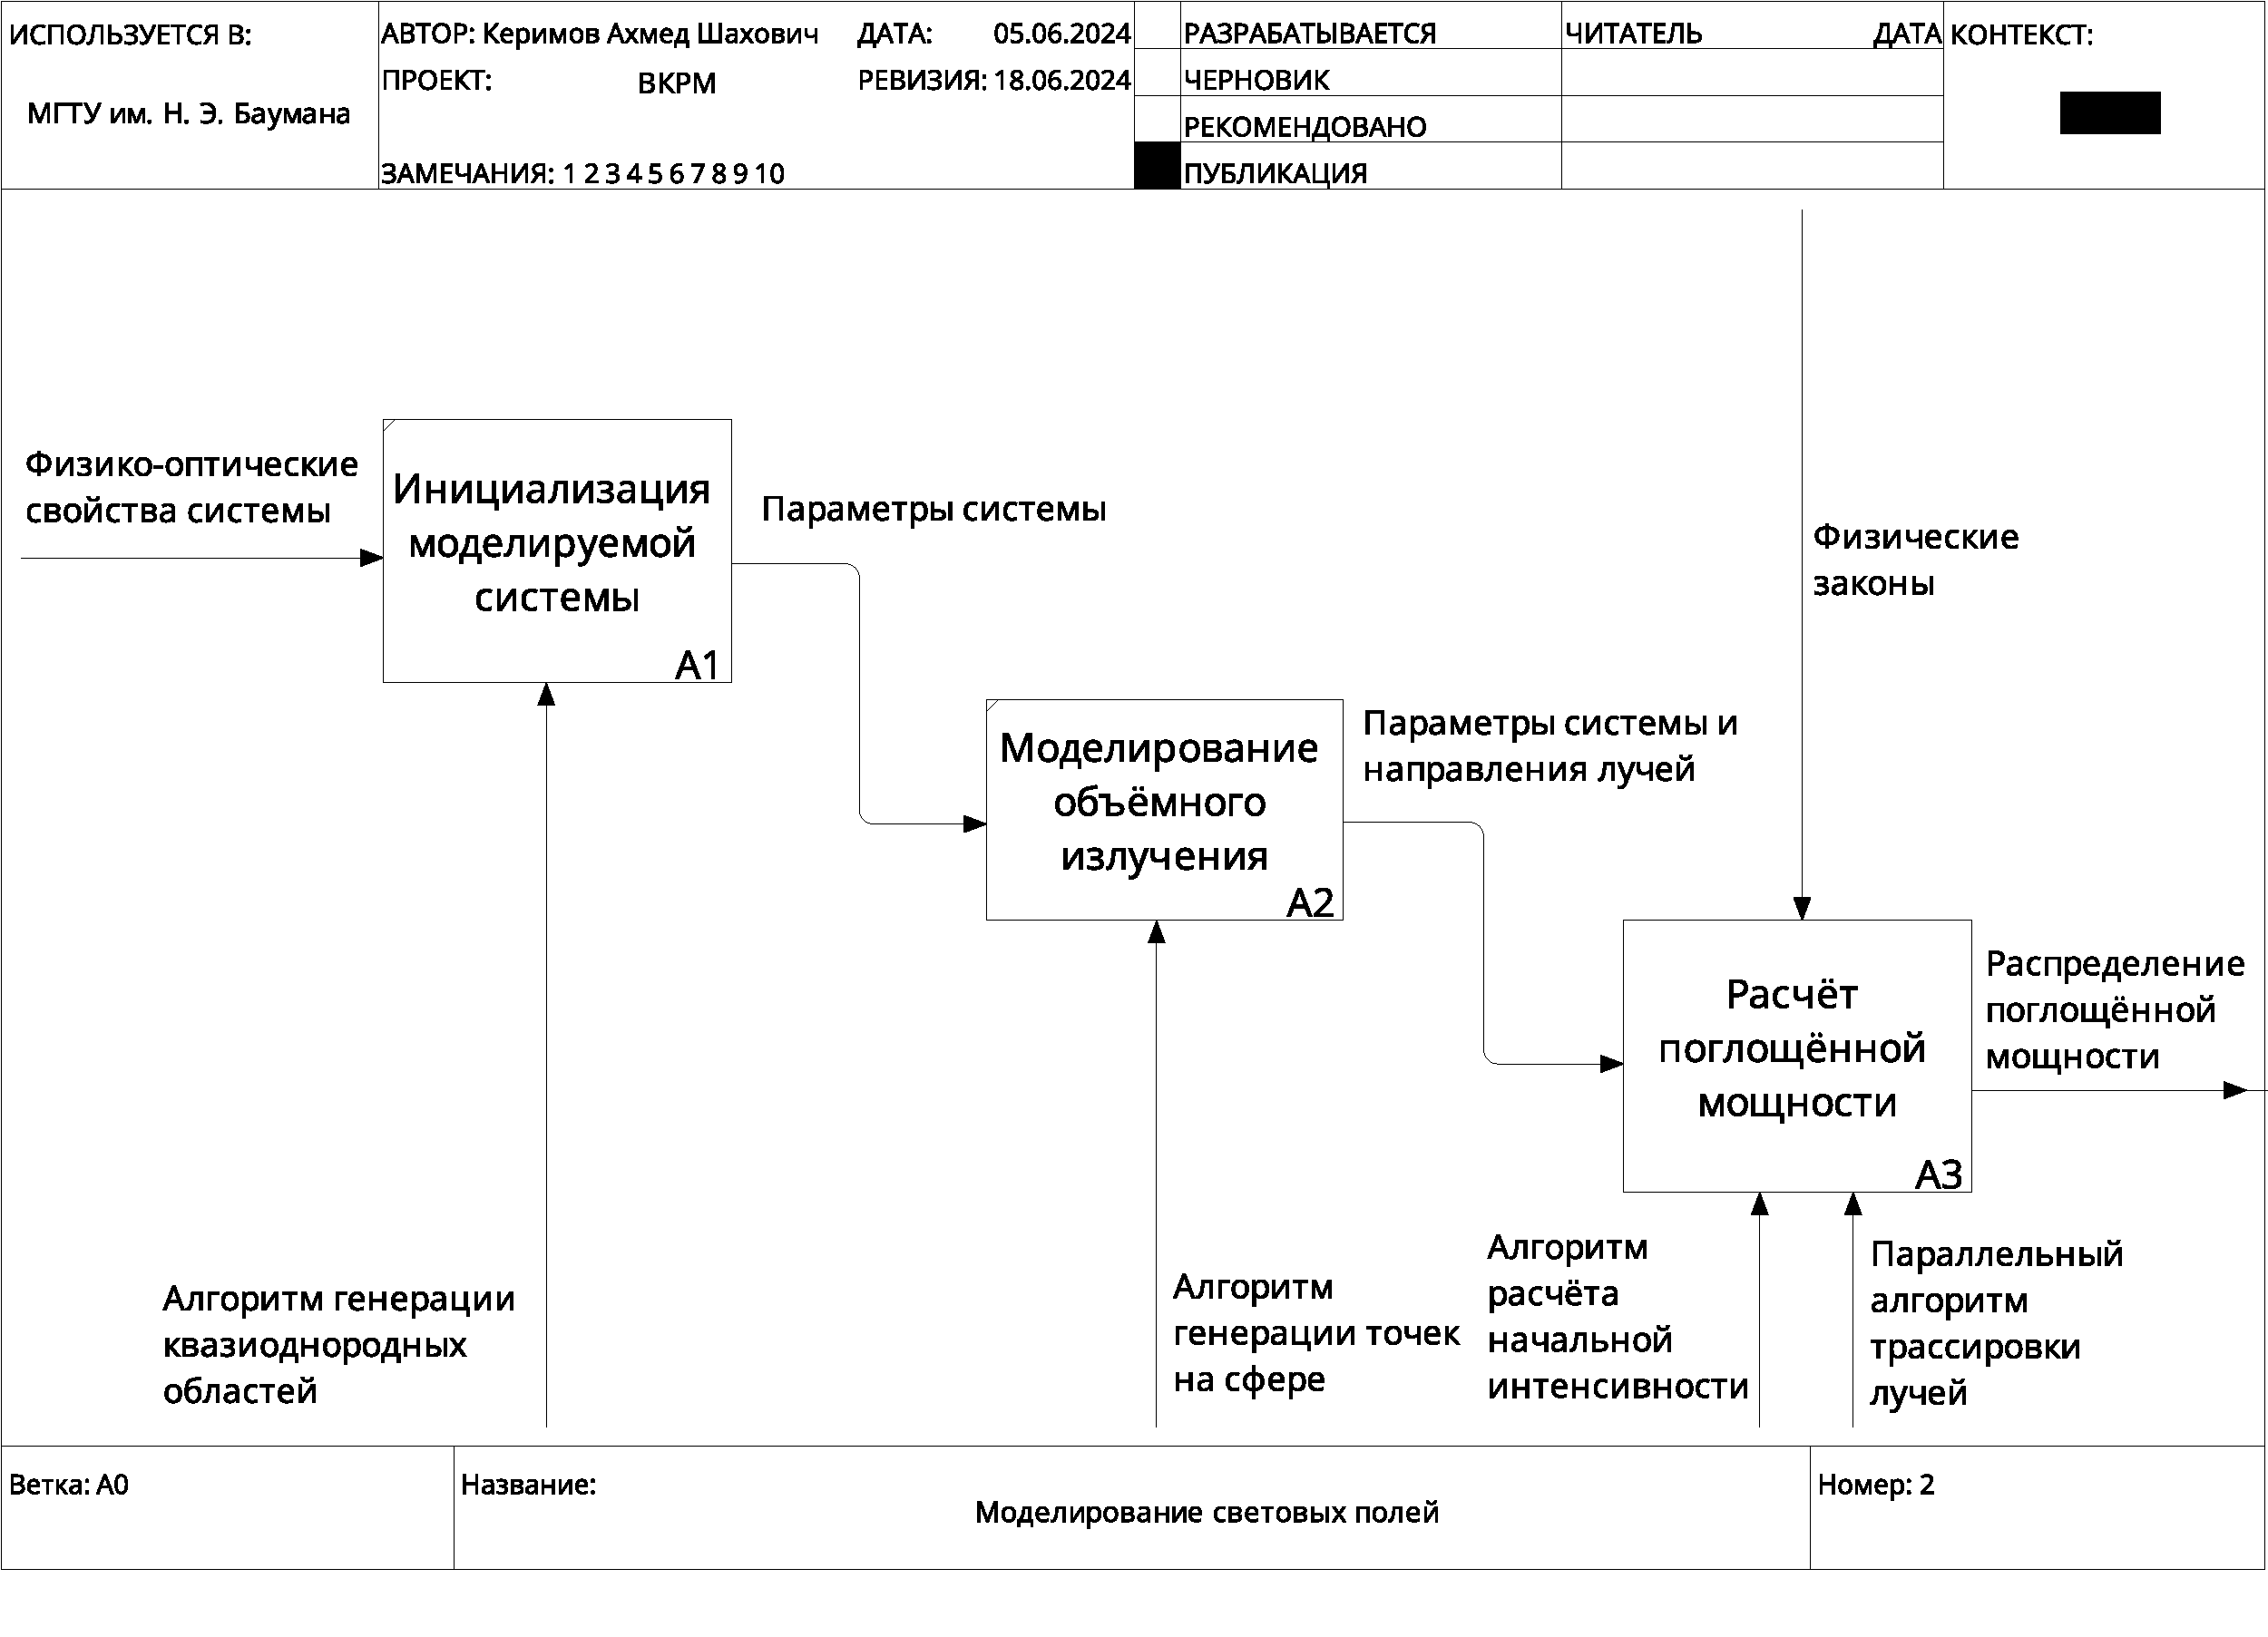
\includegraphics[width=\linewidth]{inc/img/02_A0}
		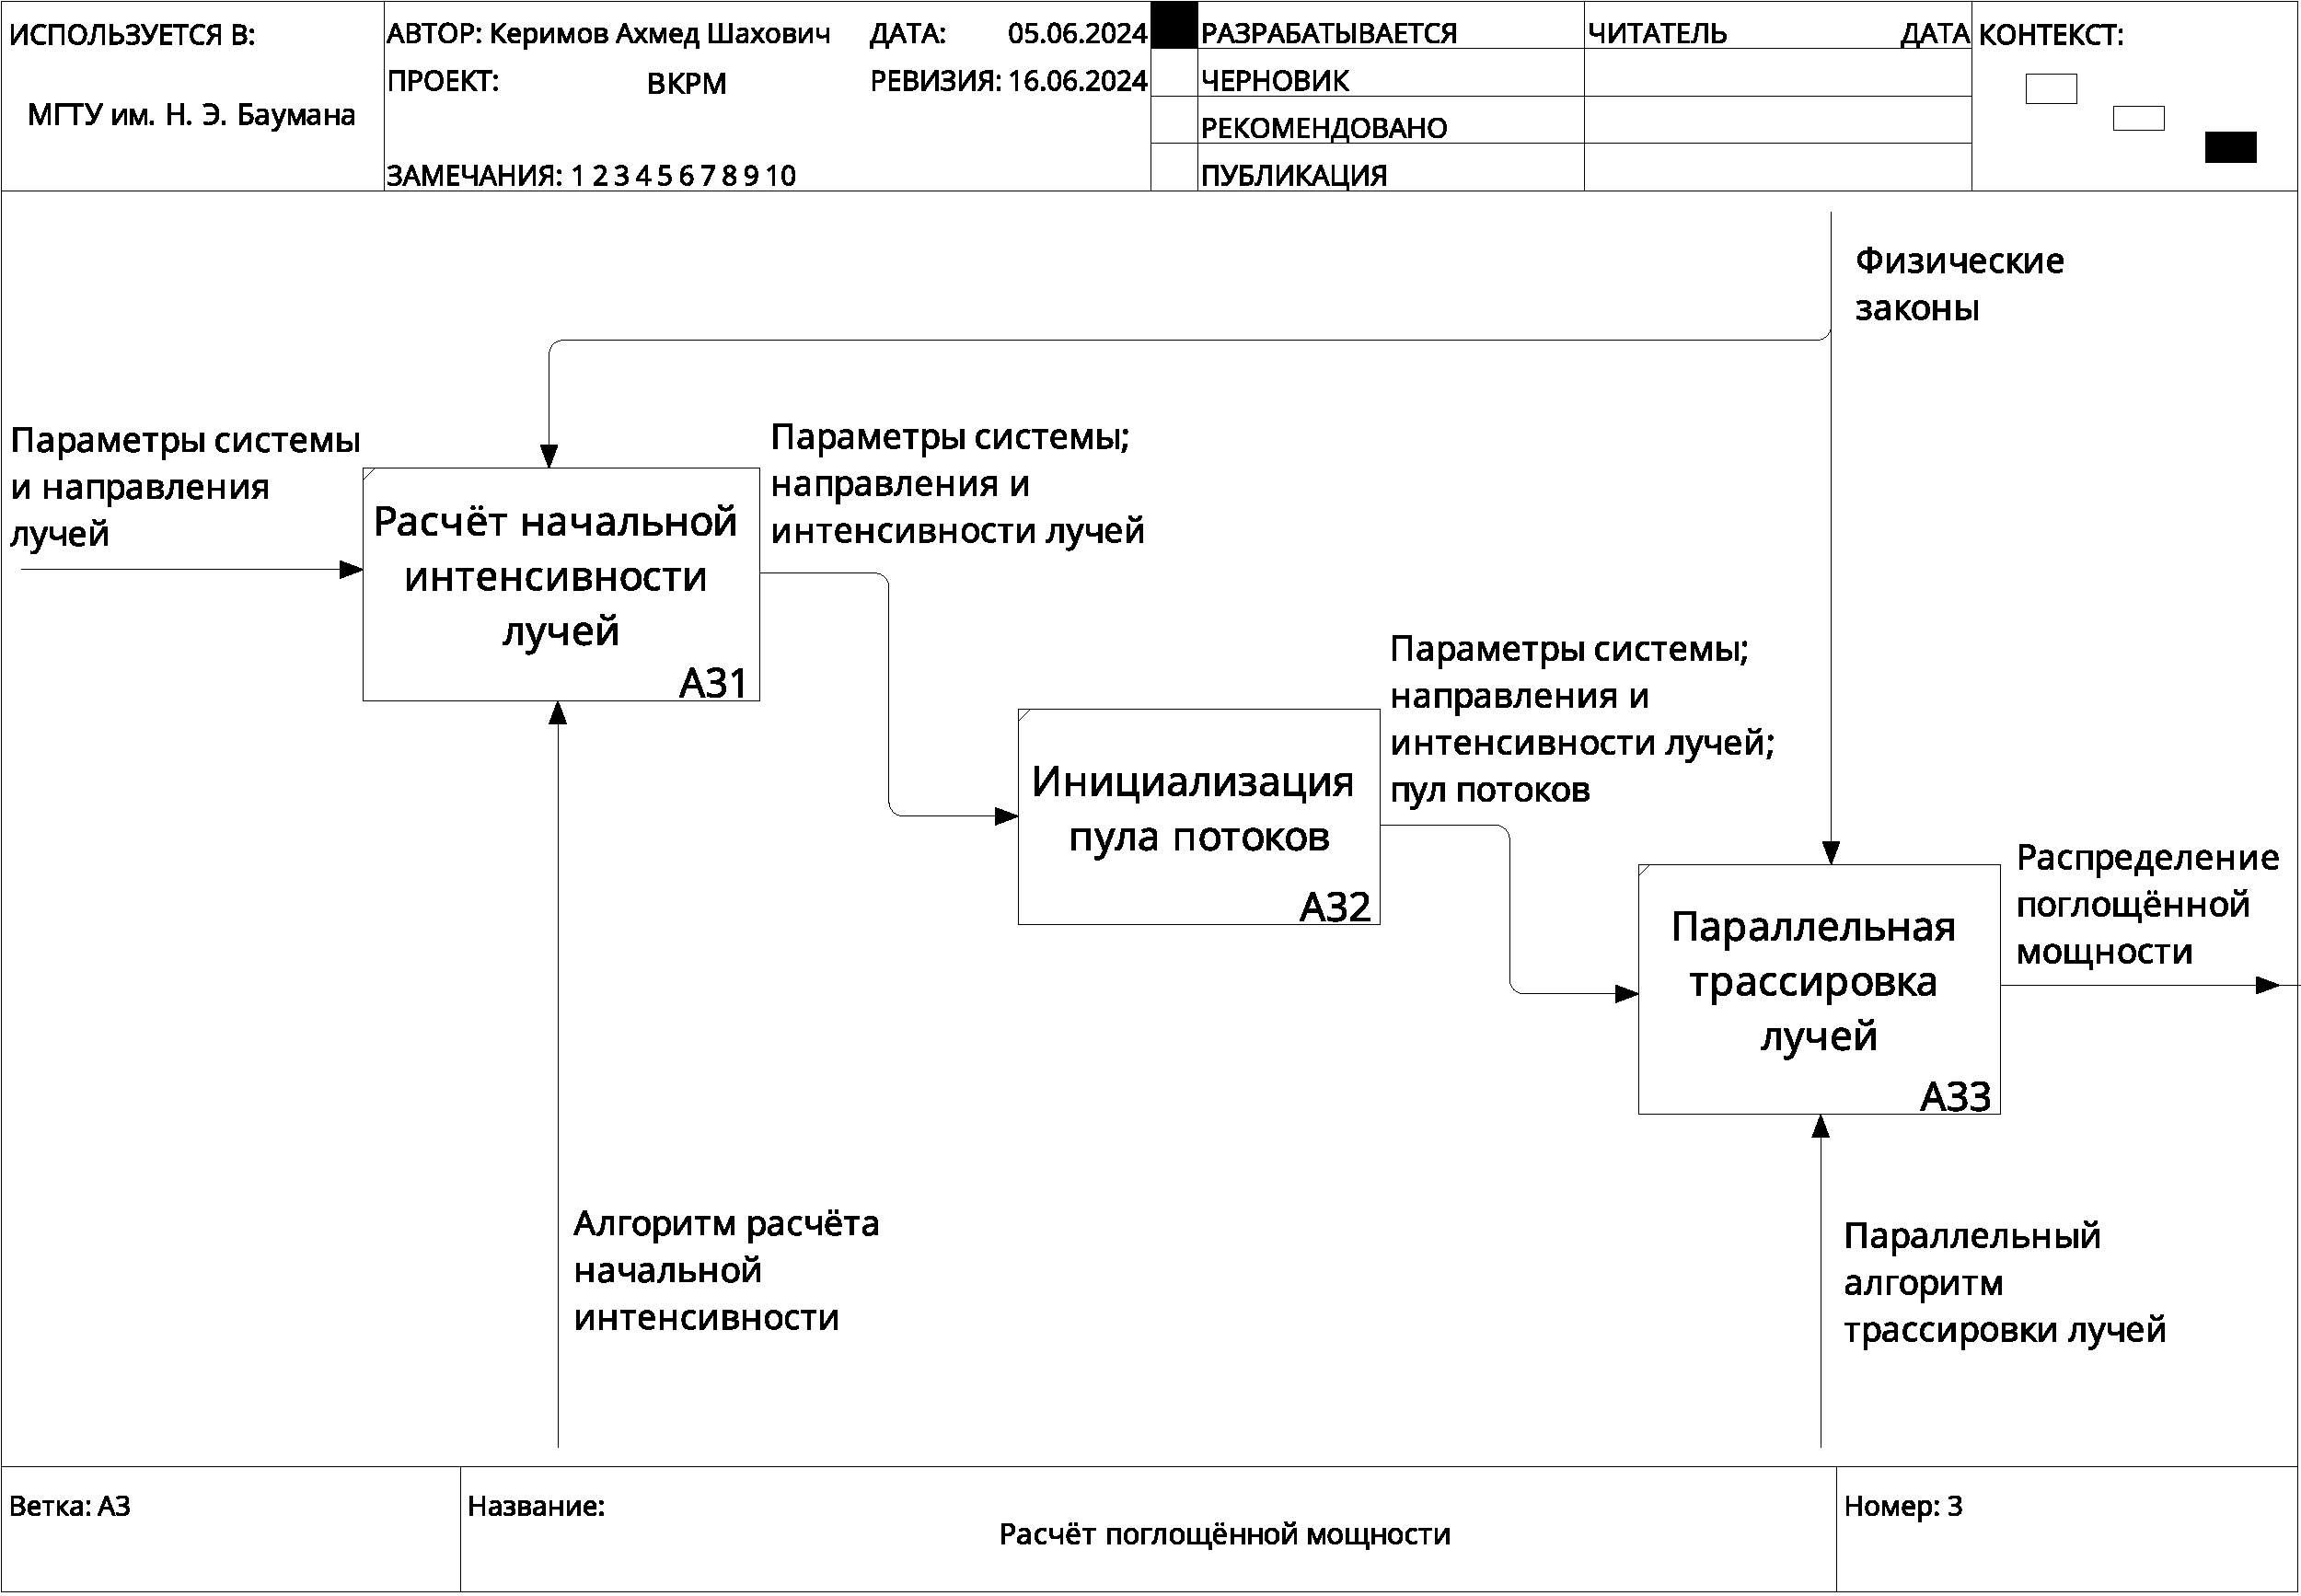
\includegraphics[width=\linewidth]{inc/img/03_A3}
	}
	\captionsetup{justification=centering}
	\caption{IDEF0 — декомпозиция веток A0 и A3}
	\label{img:02_A0_03_A3}
\end{figure}

\subsection{Инициализация моделируемой системы}

Шаг А1 (рисунок \ref{img:02_A0_03_A3}) дискретно-лучевого метода моделирования световых полей заключается в инициализации системы, а конкретно~— её сред. Цилиндрические области разбиваются на концентрические подобласти малого размера, в которых физико-оптические свойства среды считаются однородными. В качестве примера листинг \ref{alg:initialization} содержит псевдокод алгоритма разбиения области цилиндрической формы.
Аналогично происходит разбиение эллиптического цилиндра.

\begin{Algorithm}{Алгоритм разбиения цилиндра}{initialization}
	\begin{algorithmic}[1]
		\State \textbf{Вход:} $R$, $\vec C$, $N_p$ — радиус, центр и количество разбиений цилиндра; $T(z)$, $I(t)$, $k_{\text{погл}}(t)$ — функции распределения температуры от безразмерного радиуса, интенсивности излучения и коэффициента оптического поглощения от температуры
		\State \textbf{Выход:} $cylinders$, $temperatures$, $intensities$, $attenuations$ — списки цилиндров, температур, интенсивностей и коэффициентов поглощения
		\State $dr \gets R / N_p$
		\ForAll{$i$ от $1$ до $N_p$}
			\State $r \gets i \cdot dr$
			\State $Push(cylinders, Cylinder(\vec C, r))$
			\State $z \gets (r - dr / 2) / R$
			\State $t \gets T(z)$
			\State $Push(temperatures, t)$
			\State $Push(intensities, I(t))$
			\State $Push(attenuations, k_{\text{погл}}(t))$
		\EndFor
	\end{algorithmic}
\end{Algorithm}

Интенсивность $I(t)$ рассчитывается по формуле Планка \eqref{eqn:intensity-plank} при фиксированных $\nu$ и $\Delta\nu$.
Моделью распределения температуры $T(z)$ может выступать формула \eqref{eqn:xenon-temperature} при фиксированных $T_0$, $T_w$, $m$, а моделями распределения коэффициента оптического поглощения, к примеру,~— формулы \eqref{eqn:absorption-coefficient-plasma}~— \eqref{eqn:absorption-coefficient-quartz}.

\subsection{Моделирование объёмного излучения}

Так как время генерации объёмного излучения существенно меньше времени расчёта поглощённой мощности и траекторий лучей, то вместо более быстрого алгоритма генерации сферы Фибоначчи предпочтение отдано более точному алгоритму генерации каркасной сферической сетки, псевдокод которого вместе с расчётом телесных углов по каждому направлению представлен в листинге \ref{alg:wire-sphere}.

\begin{Algorithm}{Алгоритм генерация объёмного излучения}{wire-sphere}
	\begin{algorithmic}[1]
		\State \textbf{Вход:} $M$ — количество широт, $N$ — количество меридианов
		\State \textbf{Выход:} $D$ — список направлений, $\Omega$ — список, $i$-й элемент которого равен телесному углу вектора на $i$-й широте
		\State Создать пустой список векторов $D$
		\State Создать пустой список чисел $\Omega$
		\ForAll{$m$ от $0$ до $M - 1$}
			\State $y \gets (m + 1) / (M + 1)$
			\State $y_{-0,5} \gets (m + 0,5) / (M + 1)$
			\State $y_{+0,5} \gets (m + 1,5) / (M + 1)$
			\State $\phi \gets \pi y$
			\State $\phi_{-0,5} \gets \pi y_{-0,5}$
			\State $\phi_{+0,5} \gets \pi y_{+0,5}$
			\State $h \gets \cos{\phi_{-0,5}} - \cos{\phi_{+0,5}}$
			\State $S \gets 2\pi h$
			\State $\Delta\Omega \gets S / 1^2$
			\State $Push(\Omega, \Delta\Omega))$
			\ForAll{$n$ от $0$ до $N - 1$}
				\State $x \gets n / N$
				\State $\theta \gets 2 \pi x$
				\State $\overrightarrow{dir} \gets (\cos\theta \sin\phi, \sin\theta \sin\phi, \cos\phi)$
				\State $Push(D, \overrightarrow{dir})$

			\EndFor
		\EndFor
	\end{algorithmic}
\end{Algorithm}

\subsection{Расчёт начальной интенсивности лучей}

Равновесная интенсивность излучения $I_{\text{р}}$ в точке среды определяется по формуле Планка \eqref{eqn:intensity-plank}.

Интенсивность излучения, прошедшего малый участок поглощающей среды длины $\Delta l$, в пределах которой её физико-оптические свойства можно считать однородными, рассчитывается по формуле:

\begin{equation}
	I_{\text{конечная}} = I_{\text{начальная}} \cdot e^{-k\Delta l},
\end{equation}

\noindent где $k$ — коэффициент оптического поглощения на участке $\Delta l$.

Если среда вдобавок является излучающей, то на том же участке интенсивность излучения рассчитывается по формуле:

\begin{equation}
	I_{\text{конечная}} = I_{\text{начальная}} \cdot e^{-k\Delta l} + I_{\text{р}}\left(1 - e^{-k \Delta l} \right).
\end{equation}

В общем виде расчёт интенсивности луча, прошедшего путь длины $l$, записывается соотношением:

\begin{equation}
	\label{eqn:intensity-general-form}
	I = \int\displaylimits_0^l k(l') I_{\text{р}}(l') \cdot \exp{\left( -\int\displaylimits_{l'}^{l} k(l'') \,\mathrm dl'' \right)} \,\mathrm dl'.
\end{equation}

Если рассматриваемая неоднородная система является цилиндрически симметричной, то вместо ресурсоёмкого моделирования излучения из $N_p$ внутренних точек объёма его можно произвести всего из 1 точки на поверхности излучающей среды, предварительно рассчитав веса лучей по формуле \eqref{eqn:intensity-general-form}.

В таком случае интенсивность луча необходимо рассматривать как удельную, то есть через поток, проходящий сквозь единичную площадку на поверхности цилиндра:

\begin{equation}
	\hat I = I \cos{\gamma} \,\mathrm d\Omega,
\end{equation}

\noindent где $\gamma$ — угол между нормалью к поверхности и направлением луча, $\mathrm d\Omega$ — телесный угол.

Если формировать поток излучения в какой-либо точке поверхности бесконечного по оси Z цилиндра с наибольшей координатой X, то расчёт удельной интенсивности упростится: $\cos{\gamma}$ станет численно равен компоненту $D_x$ вектора направления луча $\vec D$.

В листинге \ref{alg:initial-intensity} представлен псевдокод алгоритма расчёта начальной интенсивности излучения на поверхности цилиндра.

\begin{Algorithm}{Алгоритм расчёта начальной интенсивности}{initial-intensity}
	\begin{algorithmic}[1]
		\State \textbf{Вход:} $C$, $J$, $K$ — список цилиндров, равновесных интенсивностей и коэффициентов поглощения, $\vec P$, $\vec D$, $\Delta\Omega$ ~— положение, направление и телесный угол луча на поверхности
		\State \textbf{Выход:} $I$ — начальная интенсивность луча на поверхности
		\State $I \gets 0$
		\State Найти точку пересечения $\vec A$ луча $(\vec P, - \vec D)$ с последним цилиндром
		\While{$\vec A \neq \vec P$}
			\State $\vec B \gets$ точка пересечения луча $(\vec A, \vec D)$ с ближайшим цилиндром
			\State $i \gets$ индекс ближайшего цилиндра
			\State $dr \gets |\overrightarrow{AB}|$
			\State $exp \gets e^{-K_i \cdot dr}$
			\State $I \gets I \cdot exp + J_i \cdot (1 - exp)$
			\State $\vec A \gets \vec B$
		\EndWhile
		\State $I \gets I \cdot \Delta\Omega \cdot D_x$
	\end{algorithmic}
\end{Algorithm}

\subsection{Параллельная трассировка лучей}

На рисунке \ref{img:worker} представлена схема алгоритма параллельной трассировки лучей.

\imgh{width=\linewidth}{worker}{Схема алгоритма параллельной трассировки лучей}

На рисунке \ref{img:ray-tracing} представлена схема алгоритма трассировки луча:
\begin{itemize}
	\item поиск ближайшей поверхности пересечения — поиск поверхности с наименьшим значением $t^+$: \eqref{eqn:cylinder-possible-t}, \eqref{eqn:elliptic-cylinder-possible-t}, схема алгоритма представлена на рисунке \ref{img:nearest-surface};
	\item геометрическое отражение: \eqref{eqn:reflection};
	\item преломление: \eqref{eqn:refraction-begin} — \eqref{eqn:refraction-end};
	\item перерасчёт интенсивности: \eqref{eqn:intensity-begin} — \eqref{eqn:intensity-end}.
\end{itemize}

% TODO(a.kerimov): Fix grammar
\imgh{width=\linewidth}{ray-tracing}{Схема алгоритма трассировки луча}

\imgh{width=\linewidth}{nearest-surface}{Схема алгоритма поиска ближайшей поверхности пересечения}

\section*{Выводы}

В конструкторском разделе выпускной квалификационной работы был разработан дискретно-лучевой метод моделирования световых полей в системах с неоднородными поглощающими и излучающими средами на основе параллельных вычислений.

Метод был декомпозирован на этапы, каждый из которых был описан по шагам с указанием входных и выходных параметров.

% Число базовых классификаторов было решено определить в ходе работы над исследовательским разделом.
